% !TeX root = RJwrapper.tex
\title{A review of R neural network packages (with NNbenchmark)\(:\) accuracy
and ease of use}
\author{by Salsabila Mahdi, Akshaj Verma, Christophe Dutang, Patrice Kiener, John C. Nash}

\maketitle


\hypertarget{abstract}{%
\subsection{Abstract}\label{abstract}}

In the last three decades, neural networks (NN) have evolved from an
academic topic to a common scientific computing tool. CRAN currently
hosts approximately 80 packages in May 2020 involving neural network
modeling, some offering more than one algorithm. However, to our
knowledge, there is no comprehensive study which checks the accuracy,
the reliability and the ease-of-use of those NN packages.

In this paper, we attempted to test this rather large number of packages
against a common set of datasets with different levels of complexity,
and to benchmark and rank them with certain metrics.

Restricting our evaluation to regression algorithms applied on the
one-hidden layer perceptron and ignoring those for classification or
other specialized purposes, there were approximately 60
package::algorithm pairs left to test. The criteria used in our
benchmark were: (i) the accuracy, i.e.~the ability to find the global
minima on 13 datasets, measured by the Root Mean Square Error (RMSE) in
a limited number of iterations; (ii) the speed of the training
algorithm; (iii) the availability of helpful utilities; (iv) and the
quality of the documentation.

We have attempted to give a score for each evaluation criterion and to
rank each package::algorithm pair in a global table. Overall, 15 pairs
are considered accurate and reliable and can be recommended for daily
usage. Most others should be avoided as they are either less accurate,
too slow, too difficult to handle, or have poor or no documentation.

To carry out this work, we developed various codes and templates, as
well as the NNbenchmark package used for testing. This material is
available at \url{https://akshajverma.com/NNbenchmarkWeb/index.html} and
\url{https://github.com/pkR-pkR/NNbenchmark}, and can be used to verify
our work and, we hope, improve both packages and their evaluation.
Finally, we provide some hints and features to guide the development of
an idealized neural network package for R.

\hypertarget{introduction}{%
\subsection{Introduction}\label{introduction}}

The R Project for Statistical Computing (\url{www.r-project.org}), as
any opensource platform, relies on its contributors to keep it up to
date. Neural networks (NN), inspired on the brain's own connections
system, are a class of models in the growing field of machine learning
for which R has a number of tools. During the last 30 years, neural
networks have evolved from an academic topic to a common tool in
scientific computing. Previously, neural networks were often considered
theoretically instead of pragmatically, partly because the algorithms
used were computationally demanding.

As a convenience in the general conversation, the same term is used in a
generic manner for different model structures and applications:
multilayer perceptron for regression, multilayer perceptron for
classification, multilayer perceptron for specialized applications,
recurrent neural network for autoregressive time series, convolutional
neural networks for dimension reduction and pattern recognition, and
even deep neural networks for image or voice recognition. Most of the
above types of neural networks can be found in R packages hosted on CRAN
but without any warranty about the accuracy or the speed of computation.
This is an issue as many poor algorithms are available in the literature
and hence poor packages are implemented on CRAN.

A neural network algorithm requires complicated calculations to improve
the model control parameters. As with other optimization problems, the
gradient of the chosen cost function that indicates the lack the model's
suitability is sought. This lets us improve the model by changing the
parameters in the negative gradient direction. Parameters for the model
are generally obtained using part of the available data (a training set)
and tested on the remaining data. Modern software allows much of this
work, including approximation of the gradient, to be carried out without
a large effort by the the user.

The training process can generally be made more efficient if we can also
approximate second derivatives of the cost function, allowing us to use
its curvature via the Hessian matrix. There are a large number of
approaches, of which quasi-Newton algorithms are perhaps the most common
and useful. Within this group, methods based on the
Broyden-Fletcher-Goldfarb-Shanno (BFGS) algorithm for updating the
(inverse) Hessian approximation provide several well-known examples. In
conducting this study, we believed that these second-order algorithms
would perform better than first-order methods for fit-in-memory
datasets.

Regardless of our belief, we wished to be able to conduct a thorough
examination of these training algorithms in R. There are many packages,
but barely any information to allow comparison. Our work, reported here,
aims to provide a framework for benchmarking neural network packages. We
restrict our examination to packages for R, and in this report focus on
those that provide neural networks of the perceptron type, that is, one
input layer, one normalized layer, one hidden layer with a nonlinear
activation function that is usually the hyperbolic tangent \(\tanh()\),
and one output output layer. Moreover, We restricted our evaluation to
one-hidden layer perceptron for regression and ignored those for
classification or other specialized purposes. The criteria used in our
benchmark were: (i) the accuracy, i.e.~the ability to find the global
minima on 13 datasets in a limited number of iterations; (ii) the speed
of the training algorithm; (iii) the availability of helpful utilities;
(iv) and the quality of the documentation.

\hypertarget{neural-networks-the-perceptron}{%
\section{Neural Networks: the
perceptron}\label{neural-networks-the-perceptron}}

Here, we give a short description of the one hidden layer perceptron. As
the ``layer'' term suggests it, some terms come from the representation
of graphs whereas some other terms come from the traditional literature
on nonlinear models.

Using the graph description, a one-hidden layer neural network is made
of 3 parts: (i) the layer of the input(s), (ii) the hidden layer which
consists of independent neurons, each of them performing two operations:
a linear combination of the inputs plus an offset, then a nonlinear
function applied on this linear combination. (iii) the layer of the
output(s) which is a linear combination of the output of the nonlinear
functions in the hidden layer.

The nonlinear function used in the hidden layer must have the following
four properties: continuous, differentiable, monotonic, bounded. The
logistic (\(\text{invlogit}\)), the hyperbolic tangent (\(\tanh\)) and
the arctangent (\(\text{atan}\)) functions are the usual candidates. The
above description has a simple mathematical equivalence. Let us give two
examples.

The model
\(y = a_1 + a_2\times \tanh(a_3 + a_4\times x) + a_5\times \tanh(a_6 + a_7\times x) + a_8\times \tanh(a_9 + a_{10}\times x)\)
describes a neural network (Fig. 1a) with one input, three hidden
neurons, one output model where \(x\) is the input, \(\tanh()\) is the
activation function, \(y\) is the output and \(a_1,\dots,a_{10}\) are
the parameters.

The model
\(y = a_1 + a_2\times \text{atan}(a_3 + a_4\times x_1 + a_5\times x_2 + a_6\times x_3 + a_7\times x_4 + a_8\times x_5) + a_9\times \text{atan}(a_{10} + a_{11}\times x_1 + a_{12}\times x_2 + a_{13}\times x_3 + a_{14}\times x_4 + a_{15}\times x_5) + a_{16}\text{atan}(a_{17} + a_{18}\times x_1 + a_{19}\times x_2 + a_{20}\times x_3 + a_{21}\times x_4 + a_{22}\times x_5)\)
describes a neural network (Fig. 1b) with five inputs, three hidden
neurons, one output model where \(x\) is the input, \(\text{atan}()\) is
the activation function, \(y\) is the output and \(a_1,\dots,a_{22}\)
are the parameters.

In order to get large gradients at the first steps of the training
algorithm, it is recommended to use normalized inputs and normalized
outputs (Fig. 1c), odd functions like the hyperbolic tangent function or
the arctangent function, and small random values to initialize the
parameters, for instance extracted from a centered Gaussian
\(\mathcal N(0, 0.1)\) distribution. Such good practices help find good
local minima and possibly the global minimum.

\begin{figure}
    \centering
    \begin{subfigure}[b]{0.242\textwidth}
        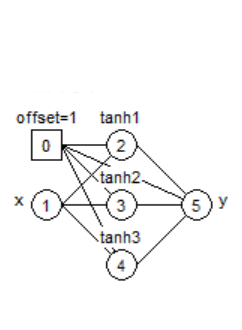
\includegraphics[width=\textwidth]{RN3a2.png}
        \caption{NN 1-3-1}
        \label{fig:N131}
    \end{subfigure}
    ~ 
    \begin{subfigure}[b]{0.250\textwidth}
        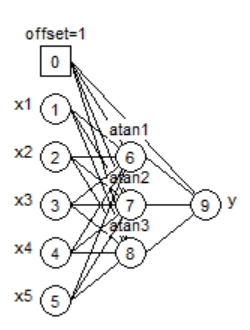
\includegraphics[width=\textwidth]{RN3b2.png}
        \caption{NN 5-3-1}
        \label{fig:N531}
    \end{subfigure}
    ~ 
    \begin{subfigure}[b]{0.396\textwidth}
        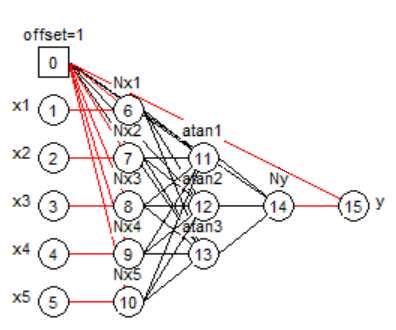
\includegraphics[width=\textwidth]{RN3c2.png}
        \caption{NN 5-5N-3-1N-1}
        \label{fig:N55311}
    \end{subfigure}
    \caption{Three neural networks}
\end{figure}

The dataset used for the training is assumed to have a number of rows
much larger than the number of parameters. While ``much larger'' is
subject to discussion, values of 3 to 5 are generally accepted (in
experimental design, some iterative strategies start with a dataset
having a number of distinct experiments equal to 1.8 times the number of
parameters and then increase the number of experiments to finetune the
model).

It is rather clear from the mathematical formula above that neural
networks of perceptron type are nonlinear models and require for their
parameter estimation some training algorithms that can handle (highly)
nonlinear models. Indeed, the intrinsic and parametric curvatures of
such models are usually very high and, with so many parameters, the
Jacobian matrix might exhibit some collinearities between its columns
and become nearly singular. As a result, appropriate algorithms for such
dataset::model pairs are rather limited and well-known. They pertain to
the class of second-order algorithms such as the BFGS algorithm which is
Quasi-Newton in how it updates the approximate inverse Hessian or the
Levenberg-Marquardt algorithm which stabilizes the Gauss-Newton search
direction at every iteration.

Unfortunately, due to some educative tools on the backpropagation and an
initial literature on the gradient in the early researches and more
recently on the ``deep neural networks'' that manipulate ultra-large
models with hundreds or thousands parameters and sometimes more
parameters than examples in the datasets, many papers emphasize the use
of first-order gradient algorithms and many R packages have implemented
such algorithms. In the case of the perceptron, we contend this is an
error, and provide evidence to that effect in this paper.

\hypertarget{methodology}{%
\section{Methodology}\label{methodology}}

\hypertarget{convergence-and-termination}{%
\subsection{Convergence and
termination}\label{convergence-and-termination}}

Most of the package:algorithm pairs try to minimize the root mean
squared error (RMSE) during the training step. Two exceptions are the
brnn package which minimizes the RMSE plus the sum of the parameters,
hence the name Bayesian Regularized Neural Network, and the qrnn package
which performs quantile regression. For all packages, the datasets were
learnt as a whole and without any weighting scheme to favour one part of
the datasets. There was no validation subset or test subset as the
purpose of our study is just to verify the ability to reach good minima.

When training neural networks, we attempt to tune a set of
hyperparameters so that the root mean squared error (RMSE) is minimized.
When our method for such adjustment can no longer reduce the RMSE, we
say that the given algorithm terminated. We consider the method to have
\textbf{converged} when termination is not due to some exceptional
situation and the final RMSE value is relatively small\footnote{We do
  not choose the mean absolute error (MAE) for overall ranking nor for
  convergence testing as there is a lack of consensus in the literature,
  see e.g.~\citep{willmott2005advantages,chai2014root}.}. In practice,
some algorithms require that we stop the optimization process in
exceptional situations (e.g., a divide by zero), or a pre-set limit on
the number of steps or a maximum elapsed time is reached.

More precisely, second-order algorithms are all set to a maximum of 200
iterations. On the other hand, first-order algorithms were set to
several values, depending on how well and how fast they converged:
\texttt{maxit1storderA=1000} iterations, \texttt{maxit1storderB=10000}
iterations, and \texttt{maxit1storderC=100000} iterations. The full list
of the maximum iteration number per package:algorithm is given in
Appendix C. It can be seen that we were unable to completely harmonize
the hyperparameters as an appropriate learning rate differed between
packages, despite the algorithm being similarly named.

\hypertarget{performance}{%
\subsection{Performance}\label{performance}}

We measure \textbf{performance} primarily by relative computing time
between methods on a particular computing platform. We could also count
measures of iterations, function evaluations or similar quantities that
indicate the computing effort. We note that differences in machine
architecture and in the attached libraries (e.g., BLAS choices for R)
will modify our measures. We are putting our tools on a Github
repository so that further evaluation can be made by ourselves and
others as hardware and software evolves.

The resulting files in our repository were mostly generated by one of us
(SM) on a Windows system build 10.0.18362.752 with an i7-8750H CPU, an
Intel(R) UHD Graphics 630 and NVIDIA GeForce GTX 1060 chip, and 16 GB of
RAM.

\hypertarget{phase-1---preparation-of-benchmark-datasets}{%
\subsection{Phase 1 - Preparation of benchmark
datasets}\label{phase-1---preparation-of-benchmark-datasets}}

\hypertarget{datasets}{%
\subsubsection{Datasets}\label{datasets}}

A non-iterative calculation such as Ordinary Least Squares cannot
generally be used to model all the datasets in our evaluation set.
Varying levels of difficulty in modeling the different data sets are
intended to allow us to further classify different algorithms and the
packages that implement them. Sonja Surjanovic and Derek Bingham of
Simon Fraser University created a useful website from which three of the
multivariate datasets were drawn. We note the link, name and difficulty
level of the three datasets:\\
- \url{http://www.sfu.ca/~ssurjano/fried.html} (Friedman - average)\\
- \url{http://www.sfu.ca/~ssurjano/detpep10curv.html} (Dette - medium)\\
- \url{http://www.sfu.ca/~ssurjano/ishigami.html} (Ishigami - high)

The other multivariate dataset, Ref153, was used to teach neural
networks at ESPCI from 2003 to 2013 and is available in the software
Neuro One at \url{http://www.inmodelia.com/software.html}

Three of the univariate datasets we used were taken from a website of
the US National Institute for Standards and Technology (NIST):
\url{https://www.itl.nist.gov/div898/strd/nls/nls_main.shtml}. (Gauss1 -
low; Gauss2 - low; Gauss3 - average)

Univariate datasets Dmod1, Dmod2 are \ldots{}

Dreyfus1 is a pure neural network which has no error. This can make it
difficult for algorithms that assume an error exists. Dreyfus2 is
Dreyfus1 with errors. Both are considered to be of low difficulty and
usually appeared in the first slides when used to teach neural networks
at ESPCI from 1991 to 2013 (\url{https://www.neurones.espci.fr/})

The last univariate dataset, NeuroOne, was also used to teach the same
course and is now available in the software Neuro One.

Finally, we also consider a Simon Wood test dataset, used in
\citep{wood2011fast} for benchmarking generalized additive models.
Precisely, we consider a generation of Gaussian random variates \(Y_i\),
\(i=1,\dots,n\) with the mean \(\mu_i\) defined as \[
\mu_i = 1+ f_0(x_{i,0})+f_1(x_{i,1})+f_2(x_{i,2})+f_3(x_{i,3})
+f_4(x_{i,4})+f_0(x_{i,5})
\] and standard deviation \(\sigma=1/4\) where \(f_j\) are Simon Wood's
smooth functions defined in Appendix B, \(x_{i,j}\) are uniform variates
and \(n=20,000\).

\hypertarget{packages}{%
\subsubsection{Packages}\label{packages}}

Using \CRANpkg{RWsearch} \citep{R-RWsearch} we sought to automate the
process of searching for neural network packages. All packages that have
``neural network'' as a keyword in the package title or in the package
description were included. In May 2020, around 80 packages falls into
this category. Packages \pkg{nlsr}, \pkg{minpack.lm}, \pkg{caret} were
added because the former 2 are important implementations of second-order
algorithms while the latter is the first cited meta package in the
CRAN's task view for machine learning,
\url{https://CRAN.R-project.org/view=MachineLearning}, as well as the
dependency for some of the other packages tested. Restricting to
regression analysis left us with 49 package::algorithm pairs in 2019 and
60 package::algorithm pairs in 2020.

\hypertarget{phase-2---review-of-packages-and-development-of-a-benchmarking-template}{%
\subsection{Phase 2 - Review of packages and development of a
benchmarking
template}\label{phase-2---review-of-packages-and-development-of-a-benchmarking-template}}

From documentation and example code, we learned that not all packages
selected by the automated search fit the scope of our research. Some
have no function to generate neural networks. Others were not regression
neural networks of the perceptron type or were only intended for very
specific purposes. Basically, each package was inspected 3 times.

\begin{enumerate}
\def\labelenumi{\arabic{enumi}.}
\item
  The discard/not discard phase: depending on the package, this could be
  decided as easily as looking at the DESCRIPTION file or having to go
  through the process of making the code and seeing the results.
\item
  Benchmarking with template that was developed in 2019 and encapsulated
  in the functions of 2020, keeping notes of whether or not the package
  was easy to use.
\end{enumerate}

\textbf{Templates for Testing Accuracy and Speed}

As we inspected the packages, we developed a template for benchmarking.
The structure of this template (for each package) is as follows:

\begin{enumerate}
\def\labelenumi{\arabic{enumi}.}
\tightlist
\item
  Set up the test environment - loading of packages, setting working
  directory and options;
\item
  Summary of tested datasets;
\item
  Loop over datasets:

  \begin{enumerate}
  \def\labelenumii{\alph{enumii}.}
  \tightlist
  \item
    setting parameters for a specific dataset,
  \item
    selecting benchmark options,
  \item
    training a neural network with a tuned functions for each package,
  \item
    calculation of convergence metrics (RMSE, MAE, WAE)\footnote{We
      measure the quality of our model by RMSE, but the mean absolute
      error (MAE) and the worst absolute error (WAE) may help
      distinguish packages with close RMSE values. See Appendix A for
      definition of convergence metrics.},
  \item
    plot each training over one initial graph, then plot the best
    result,
  \item
    add results to the appropriate existing record (*.csv file) and
  \item
    clear the environment for next loop.
  \end{enumerate}
\item
  Clearing up the environment for the next package. It is optional to
  print warnings.
\end{enumerate}

To simplify this process, we developed tools in the \pkg{NNbenchmark}
package, of which the first version was created as part of GSoC 2019. In
GSoC 2020, 3 functions encapsulating the template, that had been made
generic with an extensive use of the incredible \code{do.call} function,
were added:

\begin{enumerate}
\def\labelenumi{\arabic{enumi}.}
\tightlist
\item
  In \code{trainPredict\_1mth1data} a neural network is trained on one
  dataset and then used for predictions, with several utilities. Then,
  the performance of the neural network is exported, plotted and/or
  summarized.
\item
  \code{trainPredict\_1data} serves as a wrapper function for
  trainPredict\_1mth1data for multiple methods.
\item
  \code{trainPredict\_1pkg} serves as a wrapper function for
  trainPredict\_1mth1data for multiple datasets.
\end{enumerate}

A function for the summary of accuracy and speed, \code{NNsummary}, was
also added. The package repository is
\url{https://github.com/pkR-pkR/NNbenchmark}, with package templates in
\url{https://github.com/pkR-pkR/NNbenchmarkTemplates}.

\begin{enumerate}
\def\labelenumi{\arabic{enumi}.}
\setcounter{enumi}{2}
\tightlist
\item
  summarizing or re-reviewing the tested packages utility functions \&
  documentation
\end{enumerate}

\textbf{Ease of Use Scoring}

We define an ease-of-use measure based on what we considered a user
would need when using a neural network package for nonlinear regression,
namely, utility functions and sufficient documentation.

\begin{enumerate}
\def\labelenumi{\arabic{enumi}.}
\tightlist
\item
  Utilities (1 star)

  \begin{enumerate}
  \def\labelenumii{\alph{enumii}.}
  \tightlist
  \item
    a predict function exists
  \item
    scaling capabilities exist
  \end{enumerate}
\item
  Sufficient documentation (2 stars)

  \begin{enumerate}
  \def\labelenumii{\alph{enumii}.}
  \tightlist
  \item
    the existence of useful example/vignette = (1 star)

    \begin{itemize}
    \tightlist
    \item
      clear, with regression = 2 points
    \item
      unclear, examples use iris or are for classification only = 1
      point
    \item
      no examples = 0 points
    \end{itemize}
  \item
    input/output is clearly documented, e.g., what values are expected
    and returned by a function = (1 star)

    \begin{itemize}
    \tightlist
    \item
      clear input and output = 2 points
    \item
      only one is clear = 1 point
    \item
      both are not documented = 0 points
    \end{itemize}
  \end{enumerate}
\end{enumerate}

The ease-of-use measure ranges from 0 to 3 stars.

\hypertarget{phase-3---collection-of-and-analysis-of-results}{%
\subsection{Phase 3 - Collection of and analysis of
results}\label{phase-3---collection-of-and-analysis-of-results}}

\hypertarget{results-collection}{%
\subsubsection{Results collection}\label{results-collection}}

Looping over the datasets using each package template, we collected
results in the relevant package directories in the templates repository.

\hypertarget{analysis}{%
\subsubsection{Analysis}\label{analysis}}

To rank how well a package converged and its speed, we developed the
following method:

\begin{enumerate}
\def\labelenumi{\arabic{enumi}.}
\tightlist
\item
  The results datasets are loaded into the R environment as one large
  list. The dataset names, package:algorithm names and all 10 run
  numbers, durations, and RMSE are extracted from that list.
\item
  For the duration score (DUR), the duration is averaged by dataset. 3
  criteria for the RMSE score by dataset are calculated:

  \begin{enumerate}
  \def\labelenumii{\alph{enumii}.}
  \tightlist
  \item
    The minimum value of RMSE for each package:algorithm as a measure of
    their best performance;
  \item
    The median value of RMSE for each package:algorithm as a measure of
    their average performance, without the influence of outliers;
  \item
    The spread of the RMSE values for each package which is measured by
    the difference between the median and the minimum RMSE (d51).
  \end{enumerate}
\item
  Then, the ranks are calculated for every dataset and the results are
  merged into one wide dataframe.

  \begin{enumerate}
  \def\labelenumii{\alph{enumii}.}
  \tightlist
  \item
    The duration rank only depends on the duration;
  \item
    For minimum RMSE values, ties are decided by duration mean, then the
    RMSE median;
  \item
    For median RMSE values, ties are decided by the RMSE minimum, then
    the duration mean;
  \item
    The d51 rank only depends on itself.
  \end{enumerate}
\end{enumerate}

\begin{enumerate}
\def\labelenumi{\arabic{enumi}.}
\setcounter{enumi}{3}
\tightlist
\item
  A global score for all datasets is found by a sum of the ranks (of
  duration, minimum RMSE, median RMSE, d51 RMSE) of each
  package:algorithm for each dataset.
\item
  The final table is the result of ranking by the global minimum RMSE
  scores for each package:algorithm.
\end{enumerate}

To rank how easy or not a package was to use (TO BE DISCUSSED FURTHER):
- Functionality (util): scaling, input, output, trace - Documentation
(docs): examples, structure/functions, vignettes

\hypertarget{results}{%
\section{Results}\label{results}}

Table 1 gives the RMSE and time score per package and per algorithm. The
full list of score is given in Table 2 in Appendix C.

\textbf{Tables}

\begin{Schunk}
\begin{table}

\caption{\label{tab:unnamed-chunk-2}Result from Tested Packages}
\centering
\fontsize{7}{9}\selectfont
\begin{tabular}[t]{>{\bfseries}lcclcc}
\toprule
\multicolumn{1}{c}{ } & \multicolumn{2}{c}{Individual score} & \multicolumn{1}{c}{ } & \multicolumn{2}{c}{Global score} \\
\cmidrule(l{3pt}r{3pt}){2-3} \cmidrule(l{3pt}r{3pt}){5-6}
Package & Util & Doc & Algorithm & Time & RMSE\\
\midrule
 & 1 & 3.0 & 1. ADAPTgd & 9 & 35\\

 & 1 & 3.0 & 2. ADAPTgdwm & 16 & 24\\

 & 1 & 3.0 & 3. BATCHgd & 39 & 41\\

\multirow{-4}{*}{\raggedright\arraybackslash AMORE} & 1 & 3.0 & 4. BATCHgdwm & 40 & 39\\
\cmidrule{1-6}
 & 2 & 3.0 & 5. adam & 13 & 33\\

 & 2 & 3.0 & 6. rmsprop & 14 & 28\\

\multirow{-3}{*}{\raggedright\arraybackslash ANN2} & 2 & 3.0 & 7. sgd & 11 & 42\\
\cmidrule{1-6}
 & 1 & 3.0 & 8. trainwgrad\_adam & 50 & 18\\

 & 1 & 3.0 & 9. trainwgrad\_RMSprop & 47 & 26\\

\multirow{-3}{*}{\raggedright\arraybackslash automl} & 1 & 3.0 & 10. trainwpso & 57 & 43\\
\cmidrule{1-6}
brnn & 2 & 4.0 & 11. Gauss-Newton & 8 & 14\\
\cmidrule{1-6}
 & 2 & 3.0 & 12. optim(BFGS) & 46 & 10\\

 & 2 & 3.0 & 13. pso\_psoptim & 54 & 54\\

\multirow{-3}{*}{\raggedright\arraybackslash CaDENCE} & 2 & 3.0 & 14. Rprop & 56 & 51\\
\cmidrule{1-6}
caret & 2 & 3.0 & 15. avNNet\_nnet\_optim(BFGS) & 17 & 13\\
\cmidrule{1-6}
 & 2 & 3.0 & 16. adam & 32 & 46\\

 & 2 & 3.0 & 17. gradientDescent & 52 & 58\\

 & 2 & 3.0 & 18. momentum & 53 & 56\\

\multirow{-4}{*}{\raggedright\arraybackslash deepdive} & 2 & 3.0 & 19. rmsProp & 34 & 53\\
\cmidrule{1-6}
deepnet & 1 & 3.0 & 20. BP & 23 & 18\\
\cmidrule{1-6}
elmNNRcpp & 2 & 3.0 & 21. ELM & 1 & 59\\
\cmidrule{1-6}
ELMR & 2 & 3.0 & 22. ELM & 2 & 60\\
\cmidrule{1-6}
EnsembleBase & 1 & 1.0 & 23. nnet\_optim(BFGS) & 5 & 12\\
\cmidrule{1-6}
h2o & 2 & 2.0 & 24. first-order & 51 & 11\\
\cmidrule{1-6}
 & 2 & 0.0 & 25. adadelta & 59 & 40\\

 & 2 & 0.0 & 26. adagrad & 58 & 37\\

 & 2 & 0.0 & 27. adam & 42 & 34\\

 & 2 & 0.0 & 28. adamax & 48 & 23\\

 & 2 & 0.0 & 29. nadam & 44 & 36\\

 & 2 & 0.0 & 30. rmsprop & 37 & 52\\

\multirow{-7}{*}{\raggedright\arraybackslash keras} & 2 & 0.0 & 31. sgd & 48 & 44\\
\cmidrule{1-6}
MachineShop & 1 & 3.0 & 32. nnet\_optim(BFGS) & 6 & 5\\
\cmidrule{1-6}
minpack.lm & 1 & 3.5 & 33. Levenberg-Marquardt & 15 & 24\\
\cmidrule{1-6}
 & 2 & 3.5 & 34. optimx(BFGS) & 26 & 9\\

\multirow{-2}{*}{\raggedright\arraybackslash monmlp} & 2 & 3.5 & 35. optimx(Nelder-Mead) & 32 & 47\\
\cmidrule{1-6}
 & 1 & 3.0 & 36. backprop & 37 & 50\\

 & 1 & 3.0 & 37. rprop- & 21 & 22\\

 & 1 & 3.0 & 38. rprop+ & 19 & 21\\

 & 1 & 3.0 & 39. sag & 41 & 38\\

\multirow{-5}{*}{\raggedright\arraybackslash neuralnet} & 1 & 3.0 & 40. slr & 31 & 31\\
\cmidrule{1-6}
nlsr & 1 & 4.0 & 41. NashLM & 18 & 1\\
\cmidrule{1-6}
nnet & 1 & 3.0 & 42. optim (BFGS) & 3 & 3\\
\cmidrule{1-6}
qrnn & 2 & 3.0 & 43. nlm() & 28 & 16\\
\cmidrule{1-6}
radiant.model & 2 & 2.0 & 44. nnet\_optim(BFGS) & 10 & 7\\
\cmidrule{1-6}
rminer & 2 & 3.5 & 45. nnet\_optim(BFGS) & 12 & 2\\
\cmidrule{1-6}
 & 2 & 3.0 & 46. BackpropBatch & 43 & 49\\

 & 2 & 3.0 & 47. BackpropChunk & 26 & 29\\

 & 2 & 3.0 & 48. BackpropMomentum & 25 & 30\\

 & 2 & 3.0 & 49. BackpropWeightDecay & 29 & 31\\

 & 2 & 3.0 & 50. Quickprop & 45 & 57\\

 & 2 & 3.0 & 51. Rprop & 24 & 17\\

 & 2 & 3.0 & 52. SCG & 30 & 18\\

\multirow{-8}{*}{\raggedright\arraybackslash RSNNS} & 2 & 3.0 & 53. Std\_Backpropagation & 22 & 27\\
\cmidrule{1-6}
snnR & 2 & 2.0 & 54. SemiSmoothNewton & 7 & 48\\
\cmidrule{1-6}
traineR & 1 & 2.5 & 55. nnet\_optim(BFGS) & 4 & 6\\
\cmidrule{1-6}
 & 1 & 4.0 & 56. optim(BFGS) & 35 & 4\\

 & 1 & 4.0 & 57. optim(CG) & 60 & 8\\

 & 1 & 4.0 & 58. optim(L-BFGS-B) & 36 & 15\\

 & 1 & 4.0 & 59. optim(Nelder-Mead) & 55 & 45\\

\multirow{-5}{*}{\raggedright\arraybackslash validann} & 1 & 4.0 & 60. optim(SANN) & 20 & 55\\
\bottomrule
\end{tabular}
\end{table}

\end{Schunk}

\hypertarget{discussion-and-recommendations}{%
\subsection{Discussion and
Recommendations}\label{discussion-and-recommendations}}

\hypertarget{second-order-algorithms}{%
\subsubsection{Second order algorithms}\label{second-order-algorithms}}

Of all approaches, the following second order algorithms generally
performed better in terms of convergence despite being limited to one
fifth or fewer iterations than the first order algorithms.

We note that 11 out of 15 of these package::algorithms use \code{optim}
from \CRANpkg{stats}. 2 of them, \CRANpkg{CaDENCE}`s BFGS
\citep{R-CaDENCE} and \CRANpkg{validann}'s BFGS and L-BFGS-B
\citep{R-validann}, make the call directly. However, it is not clearly
stated in \CRANpkg{CaDENCE}'s documentation that optim's BFGS method has
been chosen rather than one of the other four methods. Furthermore, the
mention of Nelder-Mead in the documentation might suggest that
\code{optim}'s Nelder-Mead method is used. Speed and variation between
results for \CRANpkg{CaDENCE} are also not as good as other packages
that use \code{optim}. This could be because \CRANpkg{CaDENCE} is
intended for probabilistic nonlinear models with a full title of
``Conditional Density Estimation Network Construction and Evaluation''.

By contrast, \CRANpkg{validann} is clearly a package that allows a user
to use all optim's algorithms. \CRANpkg{validann}::L-BFGS-B ranks mostly
lower than \CRANpkg{validann}::BFGS, despite the former method being
more sophisticated. We believe this is due to our efforts to harmonize
parameters, thereby under-utilizing the possibilities of the L-BFGS-B
algorithm. Both \CRANpkg{CaDENCE} and validann's BFGS are outperformed
by \CRANpkg{nnet}, especially in terms of speed.

\CRANpkg{nnet} \citep{R-nnet} differs from the two packages above
because it uses the C code for BFGS (\code{vmmin.c}) from \code{optim}
(converted earlier from Pascal) directly instead of calling optim from
R. This may be what allows it to be faster, but limits the optimization
to the single method. \CRANpkg{nnet} is only beaten by the Extreme
Learning Machine (ELM) algorithms in terms of speed. However, there is a
larger variation between results (see the \texttt{RMSEd51} in Appendix
C) in comparison to \CRANpkg{validann}::BFGS. We believe the different
default JN?? starting?? values are the cause of this. For instance,
\CRANpkg{nnet} uses a range of initial random weights of 0.7 while
\CRANpkg{validann} uses a value of 0.5. In spite of these results, the
real reason most authors or users are likely to choose \CRANpkg{nnet} is
because it is included in the distributed base R and is even mentioned
as the very first package in CRAN's task view for machine learning
(\url{https://CRAN.R-project.org/view=MachineLearning}).

Our research found that 6 of the 11 packages JN?? tested?? that use
optim do so through \CRANpkg{nnet}. Moreover, approximately 8 packages
not tested use it. The total number of \CRANpkg{nnet} dependencies found
through a search through the offline database of CRAN with
\CRANpkg{RWsearch} is 136 packages, although some might be using nnet
for the multinomial log-linear models, not neural networks. The packages
that use \CRANpkg{nnet} for neural networks are often meta packages with
a host of other machine learning algorithms. \CRANpkg{caret}
\citep{R-caret}, also mentioned in the taskview, boasts 238 methods with
13 different neural network packages, under a deceivingly simple name of
``Classification and Regression Training''. It has many pre-processing
utilities available, as well as other tools.

\CRANpkg{EnsembleBase} \citep{R-EnsembleBase} maybe useful for those who
wish to make ensembles and test a grid of parameters although the
documentation is rather confusing. \CRANpkg{MachineShop}
\citep{R-MachineShop} has 51 algorithms, with some additional
information about the response variable types in the second vignette,
functions for preprocessing and tuning, performance assessment, and
presentation of results. \CRANpkg{radiant.model} \citep{R-radiant.model}
has an unalterable maxit of 10000 in the original package. Perhaps the
author thought this was reasonable as the algorithm, nnet, is quite
fast. We changed this to harmonize the parameters. \CRANpkg{rminer}
\citep{R-rminer} is the only package dependent on nnet that ranks above
nnet at number 2 for minimum RMSE, and even number 1 in some runs. It
also ranks number 1 on the other accuracy measures (median RMSE, minimum
MAE, minimum WAE) and is only behind \CRANpkg{deepdive} and
\CRANpkg{minpack.lm} in terms of results that are consistent and do not
vary (RMSEd51). The difference is probably from the change of maximum
allowable weights in rminer to 10000 from 1000 in \CRANpkg{nnet}, which
is also probably the reason its fits are slower. \CRANpkg{traineR}
\citep{R-traineR} claims to unify the different methods of creating
models between several learning algorithms.

It is worth noting is that \CRANpkg{nnet} and \CRANpkg{validann} do not
have external normalization, which is especially recommended for
validann . However, some of the packages dependent on nnet do have this
capability and it is included in the scoring for ease of use. With
\pkg{NNbenchmark}, this is done through setting \code{scale = TRUE} in
the function \code{prepare.ZZ}. Note that use of scaling may complicate
the application of constraints, so not be worth the effort for some
users. Nevertheless, users might want scaling, or at least to have a
clear explanation of the method chosen to center the variables. Scaling
of both function and parameters is one of the features that
\CRANpkg{optimx} \citep{R-optimx} incorporates, as some optimization
algorithms can work significantly better on scaled problems
\citep{Nash-nlpor14}.

Of all the packages, only \CRANpkg{monmlp} \citep{R-monmlp} call
\CRANpkg{optimx}. Since the calls are for BFGS and Nelder-Mead, they
could do better to call optim() directly, though the door is open to
other optimization methods in \CRANpkg{optimx}. However, the author,
Alex J. Cannon who is also the author of \CRANpkg{CaDENCE}, has created
a package meant to fill a certain niche, namely for multi-layer
perceptrons with optional partial monotonicity constraints. GAM-style
effect plots are also an interesting feature. Another package by Cannon
is \CRANpkg{qrnn} \citep{R-qrnn} which uses yet another algorithm:
\code{nlm()}, a ``Newton-type'' algorithm, from \CRANpkg{stats}.
Although it's performance is at the bottom of second order algorithms,
sometimes even being beaten by first order algorithms, this could also
be because of the intended use of the package compared to the tests
here. \CRANpkg{qrnn} is designed for quantile regression neural
networks, with several options. Cannon has included automatic scaling
for all 3 of his packages, as is clearly documented.

\pkg{stats} also includes \code{nls()}, for nonlinear least squares,
which defaults to an implementation of the second-order algorithm
referred to as Gauss-Newton. However, in its documentation, nls warns
against ``zero-residual'' or even small residual problems.
\citep[Section 6.4.1]{Nash-nlpor14} This was one of the motivations for
\CRANpkg{nslr} \citep{R-nlsr}. nlsr uses a variant \citep{jn77ima} of
the Levenberg-Marquardt algorithm versus the plain Gauss-Newton of
nls(), and modifies the relative offset convergence criterion to avoid a
zero divide when residuals are small. \CRANpkg{minpack.lm}
\citep{minpack.lm} offers another Marquardt approach. Where
\CRANpkg{nlsr} is entirely in R, and also allows for symbolic or
automatic derivatives (which are not relevant to the present study),
\CRANpkg{minpack.lm} uses compiled Fortran and C code for some important
computations. Its structure is also better adapted to use features
already available in nls() that may be important for some uses.

However, despite the 2 packages ultimately performing well on all runs
(capable of being in the top 3 for RMSE and not slow), there are some
reasons why users might hesitate to choose them.

First, both require the full formula of the neural network including
variables and parameters. Secondly, they require good starting values to
achieve the best convergence. Notice that in Table 1, minpack.lm does
not have a high rank. This is because we removed the random Gaussian
start values we had originally used which means the default start values
of minpack.lm were not appropriate for our datasets. We suspect
\CRANpkg{nlsr}'s performance on convergence would have similarly dropped
if it was possible to use nlsr with no user-set starting values and the
author's chosen default values were inadequate. nls() deals with this by
suggesting a companion function in \CRANpkg{stats}, selfStart().
Finally, both packages were able to find better minima when the dataset
was scaled. With no starting values and no scaling, minpack.lm::nlsLM
fails on uNeuroOne but performance is better on Friedman \& Ishigami. On
the other hand, with no start values and no scaling, it fails on
everything but mFriedman, mIshigami, uDmod2, and the Dreyfus datasets.
Similarly, there is also a notable drop in performance for
\CRANpkg{nlsr} without scaling on the Gauss datasets and mRef153. To
conclude, both packages provide algorithms that are capable of doing
well on our datasets, but may not be suitable for less experienced
users. The vignettes for \CRANpkg{nlsr} and earlier book
\citep{Nash-nlpor14} may be useful.

\CRANpkg{brnn} \citep{R-brnn} is an implementation of the Gauss-Newton
algorithm in R that does not rely on nls() or nlm() from
\CRANpkg{stats}. Although it is well-documented and has good speed,
\CRANpkg{brnn}'s implementation of the Gauss-Newton algorithm still
ranks below some of the previously mentioned BFGS and
Levenberg-Marquardt tools in terms of its global minimum RMSE. We found
2 reasons that we believe to be the cause of this. First, its model uses
one parameter fewer than the other algorithms. Only datasets uDreyfus1
and uDreyfus2 which are purely 3 hidden neurons ignore the first term.
Second, \CRANpkg{brnn} does not minimize the sum of squares of the
errors but the sum of squares of the errors plus a penalty on the
parameters. In certain circumstances -- especially with an almost
singular Jacobian matrix as with mDette, mIshigami, mRef153, uGauss3,
and uNeuroOne -- this will avoid issues with highly correlated
parameters.

The only second-order algorithm which we are unable to recommended from
the results of our research is \CRANpkg{snnR} \citep{R-snnR}. It ranked
among the 10 worst algorithms for minimum RMSE out of all 60 algorithms.

\hypertarget{first-order-algorithms}{%
\subsubsection{First order algorithms}\label{first-order-algorithms}}

Packages with first order algorithms can be broadly categorized into 2
types: (a) those that allow for one hidden layer (b) those that allow
for more than one hidden layer.

A. One hidden layer

The first category is comprised of either packages that also include
second order algorithms previously discussed or packages that use the
Extreme Learning Machine algorithm. Only 2 packages include both second
order algorithms and a lower order algorithm, that is, \CRANpkg{monmlp}
and \CRANpkg{validann}. \CRANpkg{monmlp} has one algorithm besides BFGS,
that is, \CRANpkg{optimx}'s Nelder-Mead. \CRANpkg{validann} provides the
same algorithm but from \code{optim}. \CRANpkg{validann}'s
implementation is slower, as before, but ranks slightly better for
minimum RMSE. Both implementations of Nelder-Mead do not rank well in
minimum RMSE, around 40 out of 60, with similar ranks for the other
criteria. We would also caution users to avoid the other methods in
\CRANpkg{validann} from \code{optim}. From Table 1 it may appear that
\CRANpkg{validann}'s implementation of the Conjugate Gradient (CG)
algorithm finds reasonable minima and thus is a good option. It
consistently ranked in the top 15 with minimum RMSE. However, it is the
slowest algorithm of all 60 algorithms tested. Note, this includes
algorithms from packages that call external libraries outside R in
Python or Java and packages that use as much as 100,000 iterations. On
the other hand, \CRANpkg{validann}'s SANN algorithm is relatively worse
than other packages as it ranks at number 55 for minimum RMSE although
it is in the top one third for speed (rank 20).

Packages that implement the ELMR algorithm are similar to SANN from
\CRANpkg{validann} in the sense that they are faster but do not converge
as well as other package's algorithms. The 2 packages that do so,
\CRANpkg{elmNNRcpp} \citep{R-elmNNRcpp} and \CRANpkg{ELMR}
\citep{R-ELMR} are, respectively, number 1 and number 2 in the ranks for
time but 59 and 60 (bottom 2) for minimum RMSE. \CRANpkg{ELMR} converges
slightly worse on all datasets than \CRANpkg{elmNNRcpp} but has
noticeably worse performance on the Gauss datasets, especially Gauss 1.
Even increasing the amount of neurons did not lead to better convergence
for those particular datasets.

B. More than one hidden layer

Following the trend of ``deep learning'', the last 9 packages provide
the option for more than one layer with a first order learning
algorithm. Our results show that they are often either/both slower or
worse at converging than the second order algorithms with the same
amount of neurons or layers than their counterparts. We recommend
choosing better algorithms over more layers for datasets similar to the
ones we used.

Choosing more layers often comes at the expense of speed. An example of
this is the implementation of the first order algorithm in \CRANpkg{h2o}
\citep{R-h2o}. With the same numbers of neurons it already is quite slow
- coming in at 51 out of the 60 algorithms. With the default hidden
layer sizes of 2 layers, each with 200 neurons, it takes around 10
minutes on mFriedman with a minimum RMSE of 0.0022. On the other hand,
\CRANpkg{nnet} can find a minima of the error function with a minimum
RMSE of 0.0088 in less than a second with less neurons and only one
layer. Thus, despite having a ranking of 11 in minmum RMSE in the final
run, beating some of the second order algorithms, users should be wary
of the trade off. Moreover, users might hesitate as it is not actually
clear what algorithm is used . The large number of options to choose
from seem capable of changing the basic algorithm itself into what is
considered a different algorithm by other packages (example:
``adaptive\_rate: Specify whether to enable the adaptive learning rate
(ADADELTA). This option is enabled by default.'' in link, set to false
in latest run). Some users also might not want to setup Java, which is
needed, although it is not as painful to setup as some external
libraries.

By far, the hardest package to setup which called external libraries was
\CRANpkg{tensorflow} \citep{R-tensorflow} and its derivatives. In the
summer of 2019, it took quite some time to figure out how things worked.
Then the latest TensorFlow 2.2.0 became available and we hoped to be
able to use the Eager Execution provided to avoid the R Session crashing
in the summer of 2020. Unfortunately, this led to different problems
with the translation between R and Python so we could not use the 2019
code. \CRANpkg{tfestimators} \citep{R-tfestimators} also had similar
issues and is even less supported. \CRANpkg{kerasR} \citep{R-kerasR},
which provides a consistent interface to Keras, a Python API which
provides an easier use interface to TensorFlow, had the same issue. In
the end, we tested the algorithms in \CRANpkg{keras} \citep{R-keras}
with the hope that it would be able to represent the performance of the
other packages. \CRANpkg{keras} has the second amount of most
algorithms, a total of 7, with most of them being ``adaptive''
algorithms. The highest ranking algorithm for minimum RMSE is adamax at
23 and the highest ranking algorithm for speed was rmsprop at 37 (quite
slow). However, these results were achieved with a reasonable GPU so
users might want to decide on whether to use \CRANpkg{keras} based on
their own hardware specifications. Other algorithms did not perform well
in terms of minimum RMSE and the spread of RMSE represented by RMSEd51.
As \CRANpkg{keras} also has many options available, including a
convolutional layer for CNNs, more experienced users may prefer it. On
the other hand, just deciding the learning rate (the default was not
appropriate for our datasets) can be a challenge.

The default learning rates in \CRANpkg{RSNNS} \citep{R-RSNNS} were more
appropriate to use directly. \CRANpkg{RSNNS} is an example of a package
that directly wraps around an external library, the Stuttgart Neural
Network Simulator (SNNS), to provide an easy to use interface. This
library is rather large with many implementations of neural networks. It
contains the biggest number of algorithms tested at a total of 8.
Algorithms Rprop and SCG, the best for minimum RMSE, rank at 16 and 17
respectively which is pretty good for a first order algorithm. Speed for
Rprop is better but SCG's results vary less.

\CRANpkg{AMORE} \citep{R-AMORE}: It's a shame that the focus of the
paper behind this package, it's unique point, is not explained or
documented well enough. An addition of some examples using the TAO
option as the error criterium would be helpful for using the TAO-robust
learning algorithm. Note, this type of error is most useful for data
with outliers. The function for creating a dot file to use with
\url{http://www.graphviz.org} is also interesting. ADAPT algorithms
appear to perform better than the BATCH algorithms with the parameters
used in this research.

\CRANpkg{ANN2} \citep{R-ANN2}: This package's implementation of adam or
rmsprop consistently ranked in the top half for minimum RMSE which is
not bad for a first order algorithm. It's not as accurate as second
order algorithms but all its algorithms are quite fast. C++ code was
used to enhance the speed. Functions for autoencoding are included with
anomaly detection in mind.

\CRANpkg{automl} \citep{R-automl}: It would be easier to use the
algorithms if they did not rely on the beta parameters, and instead, had
an argument of their own. However, it is nice that there are notes on
what parametes have a higher tuning priority. Rather slow (highest
ranking algorithm for speed is RMSprop at 47) with good enough
convergence (highest ranking is adam at 18).

\CRANpkg{deepdive} \citep{R-deepdive}: All algorithms are very good in
terms of little variance between results (see its RMSEd51.score).
However, the results on convergence by minimum RMSE score aren't that
good with the worst being gradientDescent which ranks 3rd from the
bottom. Not a lot of exported functions. The novelty of this package is
apparently from the ``deeptree'' and ``deepforest'' functions it
provides.

\CRANpkg{deepnet} \citep{R-deepnet}: One of the better performing
implementations of the first order algorithms backpropagation, ranking
at 18 for minimum RMSE. It's also relatively fast, ranking at 23 for
speed.

\CRANpkg{neuralnet} \citep{R-neuralnet}: Considering that this is the
only package that uses 100000 iterations as its maxit parameter
(excluding BNN which is not included in the official ranks), it can be
considered as not recommended. Nonetheless, the default algorithm,
rprop+ and the similar rprop-, managed to rank 20 and 21 respectively,
out of 60 algorithms for minimum RMSE. These two also do not do bad in
terms of speed. After, in order, are slr, sag, and traditional backprop
as the worst at rank 48 out of 60 for minimum RMSE. Notes on
documentation show that is rather hard to configure this package, and
should probably not be a dependency for other packages that wish to be
more certain of the results. For simple datasets, it is less of an
issue.

\hypertarget{untested-to-do---list}{%
\subsubsection{Untested =\textgreater{} TO DO -
LIST}\label{untested-to-do---list}}

\begin{enumerate}
\def\labelenumi{\arabic{enumi}.}
\tightlist
\item
  For regression but unsuitable for the scope of our research
\item
  For time series
\item
  For classification
\item
  For specific purpose
\item
  For tools to complement NN's by other packages
\item
  Not actually neural networks
\item
  Error 
\end{enumerate}

\hypertarget{r-echofalse-messagefalse}{%
\section{```\{r echo=FALSE,
message=FALSE\}}\label{r-echofalse-messagefalse}}

Following chunk has NOT been executed

\begin{verbatim}
library(kableExtra)
options(knitr.kable.NA = '')

if(file.exists("./tables/Table2.csv")) {  
  Table2 <- read.csv("./tables/Table2.csv", sep = ";")
  Table2 <- Table2[Table2[,3] != "", ]
  Table2 <- Table2[,1:3]
}

colnames(Table2) <- c("Package", "Category", "Reason to Dsicard (Where)")



kableExtra::kable(Table2, booktabs = TRUE, centering = TRUE, longtable = TRUE,
                  caption="Review of Discarded Packages") %>%
  kable_styling(font_size=7) %>%
  column_spec(4, width = "10cm")
\end{verbatim}

\hypertarget{conclusion-and-perspective}{%
\section{Conclusion and perspective}\label{conclusion-and-perspective}}

??JN: Can we start to put in some major findings? i.e., important
positive findings, big negatives?

\hypertarget{positives-no-particular-order}{%
\subsection{Positives (no particular
order)}\label{positives-no-particular-order}}

\begin{enumerate}
\def\labelenumi{\arabic{enumi}.}
\tightlist
\item
  We are happy to note the existence of neural network packages in R
  with algorithms that converge well.
\end{enumerate}

\begin{itemize}
\tightlist
\item
  \pkg{nnet}, which uses ?? need font choice?? optim's BFGS method, is
  already often chosen to represent neural networks for packages that
  are either a collection of independent machine learning algorithms,
  ensembles, or even applications in a field such as \ldots{} ?? need to
  complete sentence??. JN??: Why is this positive? ==\textgreater{} B:
  its meant to be part of the above, because nnet's algorithm converged
  well in our tests, thus the fact that it is being used by other
  packages is a plus? See the part about nnet \& packages that depend on
  it in the results
\item
  R users have access to a wide variety of neural network methods,
  including from libraries of other programming languages and using many
  different types of algorithms. ?? have we defined hyperparameters??
  hyperparameters, and uses 
\end{itemize}

\hypertarget{negatives}{%
\subsection{Negatives}\label{negatives}}

\begin{itemize}
\tightlist
\item
  We are disappointed that many of the packages we reviewed had poor
  documentation.
\item
  It would be helpful if there were more packages with (different)
  second order algorithms. A number of the 
\item
  We often found it difficult to discover what default starting values
  were used for model parameters, or 
\end{itemize}

\hypertarget{future-work}{%
\subsection{Future work}\label{future-work}}

As the field of neural networks continue to grow, there will always be
more algorithms to validate. For current algorithms in R, our research
should be extended to encompass more types of neural networks and their
data formats (classifier neural networks, recurrent neural networks, and
so on). Different rating schemes and different parameters for package
functions can also be tried out.

\begin{itemize}
\tightlist
\item
  The dreamed NN package: Recommendation to package authors
\item
  Conclusion
\end{itemize}

\hypertarget{acknowledgements}{%
\subsection{Acknowledgements}\label{acknowledgements}}

This work was possible due to the support of the Google Summer of Code
initiative for R during years 2019 and 2020. Students Salsabila Mahdi
(2019 and 2020) and Akshaj Verma (2019) are grateful to Google for the
financial support.

\bibliography{RJreferences}

\hypertarget{appendix}{%
\section{Appendix}\label{appendix}}

\hypertarget{appendix-a}{%
\subsection{Appendix A}\label{appendix-a}}

Consider a set of observations \(y_i\) and its corresponding predictions
\(\hat y_i\) for \(i=1,\dots,n\). The three metrics used were: \[
MAE = \frac1n\sum_{i=1}^n|y_i - \hat y_i|,~
RMSE = \frac1n\sqrt{\sum_{i=1}^n(y_i - \hat y_i)^2},~
WAE = \frac1n\max_{i=1,\dots,n}|y_i - \hat y_i|.
\] These values represent the absolute, the squared and the maximum norm
of residual vectors.

\hypertarget{appendix-b}{%
\subsection{Appendix B}\label{appendix-b}}

We define five smooth functions for Simon Wood's test dataset \[
f_0=5\sin(2\pi x),~
f_1=exp(3x)-7
f_2=0.5 x^{11}(10(1 - x))^6 - 10 (10x)^3(1 - x)^{10},~
\] \[
f_3=15 \exp(-5 |x-1/2|)-6,
\] \[
f_4=2-1_{(x <= 1/3)}(6x)^3 - 1_{(x >= 2/3)} (6-6x)^3 - 
1_{(2/3 > x > 1/3)}(8+2\sin(9(x-1/3)\pi)).
\]

\hypertarget{appendix-c}{%
\subsection{Appendix C}\label{appendix-c}}

\begin{Schunk}
\begin{table}

\caption{\label{tab:unnamed-chunk-3}All convergence scores per package:algorithm}
\centering
\fontsize{8}{10}\selectfont
\begin{tabular}[t]{r>{\bfseries}llllrrrr}
\toprule
\multicolumn{2}{c}{ } & \multicolumn{3}{c}{Input parameter} & \multicolumn{2}{c}{RMSE Score} & \multicolumn{2}{c}{Other score} \\
\cmidrule(l{3pt}r{3pt}){3-5} \cmidrule(l{3pt}r{3pt}){6-7} \cmidrule(l{3pt}r{3pt}){8-9}
Num & Package:Algorithm & Input format & Maxit & Learn. rate & median & d51 & MAE & WAE\\
\midrule
1 & AMORE:DAPTgd & x \& y & 1000 & 0.01 & 25 & 8 & 26 & 21\\
2 & AMORE:DAPTgdwm & x \& y & 1000 & 0.01 & 22 & 29 & 16 & 26\\
3 & AMORE:ATCHgd & x \& y & 10000 & 0.1 & 38 & 24 & 42 & 31\\
4 & AMORE:ATCHgdwm & x \& y & 10000 & 0.1 & 33 & 14 & 37 & 27\\
5 & ANN2:dam & x \& y & 1000 & 0.01 & 27 & 27 & 28 & 21\\
\addlinespace
6 & ANN2:msprop & x \& y & 1000 & 0.01 & 25 & 33 & 27 & 23\\
7 & ANN2:gd & x \& y & 1000 & 0.01 & 37 & 22 & 36 & 29\\
8 & automl:rainwgrad\_adam & x \& y & 1000 & 0.01 & 20 & 35 & 16 & 20\\
9 & automl:rainwgrad\_RMSprop & x \& y & 1000 & 0.01 & 31 & 50 & 29 & 39\\
10 & automl:trainwpso & x \& y & 1000 & - & 41 & 49 & 41 & 38\\
\addlinespace
11 & brnn:Gauss-Newton & x \& y & 200 & - & 12 & 9 & 13 & 12\\
12 & CaDENCE:optim(BFGS) & x \& y & 200 & - & 28 & 48 & 21 & 40\\
13 & CaDENCE:pso\_psoptim & x \& y & 1000 & - & 56 & 56 & 54 & 56\\
14 & CaDENCE:Rprop & x \& y & 1000 & 0.01 & 54 & 60 & 52 & 58\\
15 & caret:avNNet\_nnet\_optim(BFGS) & x \& y & 200 & - & 10 & 21 & 11 & 9\\
\addlinespace
16 & deepdive:adam & x \& y & 10000 & 0.4 & 42 & 1 & 38 & 44\\
17 & deepdive:gradientDescent & x \& y & 10000 & 0.8 & 57 & 2 & 57 & 53\\
18 & deepdive:momentum & x \& y & 1000 & 0.8 & 52 & 3 & 53 & 51\\
19 & deepdive:rmsProp & x \& y & 1000 & 0.8 & 46 & 4 & 48 & 50\\
20 & deepnet:BP & x \& y & 1000 & 0.8 & 18 & 38 & 24 & 17\\
\addlinespace
21 & elmNNRcpp:ELM & x \& y & - & - & 59 & 55 & 59 & 59\\
22 & ELMR:ELM & fmla \& data & - & - & 60 & 53 & 60 & 60\\
23 & EnsembleBase:nnet\_optim(BFGS) & x \& y & 200 & - & 15 & 34 & 15 & 15\\
24 & h2o:first-order & "y" \& data & 10000 & 0.01 & 7 & 7 & 8 & 8\\
25 & keras:adadelta & x \& y & 10000 & 0.1 & 35 & 19 & 34 & 33\\
\addlinespace
26 & keras:adagrad & x \& y & 10000 & 0.1 & 43 & 53 & 42 & 35\\
27 & keras:adam & x \& y & 10000 & 0.1 & 28 & 44 & 30 & 25\\
28 & keras:adamax & x \& y & 10000 & 0.1 & 18 & 20 & 20 & 16\\
29 & keras:nadam & x \& y & 10000 & 0.1 & 39 & 58 & 40 & 41\\
30 & keras:rmsprop & x \& y & 10000 & 0.1 & 55 & 57 & 55 & 54\\
\addlinespace
31 & keras:sgd & x \& y & 10000 & 0.1 & 45 & 47 & 45 & 43\\
32 & MachineShop:nnet\_optim(BFGS) & fmla \& data & 200 & - & 9 & 22 & 9 & 7\\
33 & minpack.lm:Levenberg-Marquardt & full fmla \& data & 200 & - & 16 & 5 & 19 & 14\\
34 & monmlp:optimx(BFGS) & x \& y & 200 & - & 10 & 18 & 9 & 11\\
35 & monmlp:optimx(Nelder-Mead) & x \& y & 10000 & - & 47 & 45 & 44 & 47\\
\addlinespace
36 & neuralnet:backprop & fmla \& data & 100000 & 0.001 & 51 & 10 & 49 & 45\\
37 & neuralnet:rprop- & fmla \& data & 100000 & - & 21 & 42 & 21 & 18\\
38 & neuralnet:rprop+ & fmla \& data & 100000 & - & 23 & 40 & 23 & 24\\
39 & neuralnet:sag & fmla \& data & 100000 & - & 49 & 59 & 47 & 52\\
40 & neuralnet:slr & fmla \& data & 100000 & - & 39 & 37 & 39 & 46\\
\addlinespace
41 & nlsr:NashLM & full fmla \& data & 200 & - & 3 & 16 & 3 & 6\\
42 & nnet:optim (BFGS) & x \& y & 200 & - & 2 & 17 & 2 & 3\\
43 & qrnn:nlm() & x \& y & 200 & - & 14 & 25 & 7 & 36\\
44 & radiant.model:nnet\_optim(BFGS) & "y" \& data & 200 & - & 8 & 32 & 12 & 10\\
45 & rminer:nnet\_optim(BFGS) & fmla \& data & 200 & - & 1 & 6 & 1 & 1\\
\addlinespace
46 & RSNNS:BackpropBatch & x \& y & 10000 & 0.1 & 48 & 27 & 50 & 48\\
47 & RSNNS:BackpropChunk & x \& y & 1000 & - & 34 & 41 & 32 & 34\\
48 & RSNNS:BackpropMomentum & x \& y & 1000 & - & 35 & 39 & 35 & 30\\
49 & RSNNS:BackpropWeightDecay & x \& y & 1000 & - & 30 & 43 & 33 & 31\\
50 & RSNNS:Quickprop & x \& y & 10000 & - & 58 & 36 & 58 & 57\\
\addlinespace
51 & RSNNS:Rprop & x \& y & 1000 & - & 23 & 52 & 25 & 28\\
52 & RSNNS:SCG & x \& y & 1000 & - & 17 & 26 & 18 & 19\\
53 & RSNNS:Std\_Backpropagation & x \& y & 1000 & 0.1 & 32 & 31 & 31 & 36\\
54 & snnR:SemiSmoothNewton & x \& y & 200 & - & 49 & 13 & 50 & 48\\
55 & traineR:nnet\_optim(BFGS) & fmla \& data & 200 & - & 5 & 15 & 6 & 2\\
\addlinespace
56 & validann:optim(BFGS) & x \& y & 200 & - & 4 & 10 & 4 & 5\\
57 & validann:optim(CG) & x \& y & 1000 & - & 6 & 10 & 5 & 4\\
58 & validann:optim(L-BFGS-B) & x \& y & 200 & - & 13 & 30 & 14 & 13\\
59 & validann:optim(Nelder-Mead) & x \& y & 10000 & - & 44 & 45 & 46 & 42\\
60 & validann:optim(SANN) & x \& y & 1000 & - & 53 & 51 & 56 & 55\\
\bottomrule
\end{tabular}
\end{table}

\end{Schunk}

\hypertarget{appendix-d}{%
\subsection{Appendix D}\label{appendix-d}}

\begin{table}[htb!]
\begin{center}
\caption{\textbf{Review of Ommitted Packages}}
\scriptsize

\begin{tabular}{l l l l}
  \toprule
  No & Name (package)         & Category & Comment \\
  \midrule
  1  &\pkg{appnn}             & AP        & This package provides a feed forward neural network to predict\\
     &                        &           & the amyloidogenicity propensity of polypeptide sequences      \\
  2  &\pkg{autoencoder}       & AP        & This package provides a sparse autoencoder, an unsupervised   \\
     &                        &           & algorithm that learns useful features from the data its given \\
  3  &\pkg{BNN}               & RE*       & This package uses a feed forward neural network to perform    \\
     &                        &           & regression as provided in the examples, however, it is unclear\\      &                        &           & whether it fits the form of perceptron that is the scope of   \\
     &                        &           & our research. Moreover, it states that it is intended for     \\      &                        &           & variable selection. Although how exactly the package would be \\
     &                        &           & used to do so isn't accessible in the package, especially     \\
     &                        &           & considering the source code is based on .c code that users of \\
     &                        &           & R might not understand. It's performance is slow, which may   \\
     &                        &           & have to do with the 100.000 iterations it needs, although     \\
     &                        &           & quite accurate for simple datasets.                           \\
  4  &\pkg{Buddle}            & RE**      & (errors)\\
  5  &\pkg{cld2}              & 00        & \\
  6  &\pkg{cld3}              & AP        & \\
  7  &\pkg{condmixt}          & AP        & \\
  8  &\pkg{deep}              & CL        & \\
  9  &\pkg{DALEX2}            & 00        & removed keyword, included in 2019 \\
  10 &\pkg{DamiaNN}           & RE**      & (errors) exported functions, still doesn't work \\
  11 &\pkg{DChaos}            & ??        & removed keyword for some reason, need to check out! \\
  12 &\pkg{deepNN}            & RE**      & (errors) I/O weird, ragged vector array \\
  13 &\pkg{DNMF}              & AP        & \\
  14 &\pkg{evclass}           & CL        & \\
  15 &\pkg{gamlss.add}        & RE        & there is some code but dist not appropriate \\
  16 &\pkg{gcForest}          & 00        & \\
  17 &\pkg{GMDH}              & TS        & \\
  18 &\pkg{GMDH2}             & CL        & \\
  19 &\pkg{GMDHreg}           & RE*       & \\
  20 &\pkg{grnn}              & RE**      & \\
  21 &\pkg{hybridEnsemble}    & ??        & \\ 
  22 &\pkg{isingLenzMC}       & AP        & \\
  23 &\pkg{leabRa}            & ??        & \\      
  24 &\pkg{learNN}            & ??        & \\     
  25 &\pkg{LilRhino}          & AP        & \\
  26 &\pkg{neural}            & CL        & \\
  27 &\pkg{NeuralNetTools}    & UT        & tools for neural networks           \\
  28 &\pkg{NeuralSens}        & UT        & tools for neural networks           \\
  29 &\pkg{NlinTS}            & TS        & Time Series                         \\
  30 &\pkg{nnetpredint}       & UT        & confidence intervals for NN          \\
  31 &\pkg{nnfor}             & TS        & Times Series, uses neuralnet         \\
  32 &\pkg{nntrf}             & UT        & \\
  33 &\pkg{onnx}              &           & provides an open source format       \\
  34 &\pkg{OptimClassifier}   &           & choose classifier parameters, nnet   \\
  35 &\pkg{OSTSC}             &           & solving oversampling classification  \\
  36 &\pkg{passt}             &           & \\
  36 &\pkg{pnn}               &           & Probabilistic                        \\
  37 &\pkg{polyreg}           &           & polyregression as alternative to NN  \\
  38 &\pkg{predictoR}         &           & shiny interface, neuralnet           \\
  39 &\pkg{ProcData}          &           & \\
  40 &\pkg{QuantumOps}        &           & classifies MNIST, Schuld (2018), removed keyword, in 2019 \\
  41 &\pkg{quarrint}          &           & specified classifier for quarry data \\
  42 &\pkg{rasclass}          &           & classifier for raster images, nnet?  \\
  43 &\pkg{rcane}             &           & \\
  44 &\pkg{regressoR}         &           & a manual rich version of predictoR   \\
  45 &\pkg{rnn}               &           & Recurrent                            \\
  46 &\pkg{RTextTools}        &           & \\
  47 &\pkg{ruta}              &           & \\
  48 &\pkg{simpleNeural}      &           & \\
  49 &\pkg{softmaxreg}        &           & \\
  50 &\pkg{Sojourn.Data}      &           & sojourn Accelerometer methods, nnet? \\
  51 &\pkg{spnn}              &           & classifier, probabilistic            \\
  52 &\pkg{studyStrap}        &           & \\
  53 &\pkg{TeachNet}          &           & classifier, selfbuilt, slow          \\
  54 &\pkg{tensorflow}        &           & \\
  55 &\pkg{tfestimators}      &           & \\
  56 &\pkg{trackdem}          &           & classifier for particle tracking     \\
  57 &\pkg{TrafficBDE}        & RE*       & \\
  58 &\pkg{tsfgrnn}           &           & \\
  59 &\pkg{yap}               &           & \\
  60 &\pkg{yager}             & RE*       & \\
  61 &\pkg{zFactor}           & AP        & 'compressibility' of hydrocarbon gas \\
\end{tabular}
\end{center}
\end{table}

\hypertarget{appendix-e}{%
\subsection{Appendix E}\label{appendix-e}}

\begin{Schunk}
\begin{Sinput}
library(NNbenchmark)
nrep <- 3       
odir <- tempdir()

library(nnet)
nnet.method <- "BFGS"
hyperParams.nnet <- function(...) {
    return (list(iter=200, trace=FALSE))
}
NNtrain.nnet <- function(x, y, dataxy, formula, neur, method, hyperParams, ...) {
    
    hyper_params <- do.call(hyperParams, list(...))
    
    NNreg <- nnet::nnet(x, y, size = neur, linout = TRUE, maxit = hyper_params$iter, trace=hyper_params$trace)
    return(NNreg)
}
NNpredict.nnet  <- function(object, x, ...) { predict(object, newdata=x) }
NNclose.nnet    <- function() {  if("package:nnet" %in% search())
                                detach("package:nnet", unload=TRUE) }
nnet.prepareZZ  <- list(xdmv = "d", ydmv = "v", zdm = "d", scale = TRUE)

res <- trainPredict_1pkg(4:5, pkgname = "nnet", pkgfun = "nnet", nnet.method,
  prepareZZ.arg = nnet.prepareZZ, nrep = nrep, doplot = TRUE,
  csvfile = FALSE, rdafile = FALSE, odir = odir, echo = FALSE)
\end{Sinput}

\includegraphics{2020-rticle_files/figure-latex/unnamed-chunk-4-1} 
\includegraphics{2020-rticle_files/figure-latex/unnamed-chunk-4-2} \end{Schunk}


\address{%
Salsabila Mahdi\\
Universitas Syiah Kuala\\
JL. Syech Abdurrauf No.3, Aceh 23111, Indonesia\\
}
\href{mailto:bila.mahdi@mhs.unsyiah.ac.id}{\nolinkurl{bila.mahdi@mhs.unsyiah.ac.id}}

\address{%
Akshaj Verma\\
Manipal Institute of Technology\\
Manipal, Karnataka, 576104, India\\
}
\href{mailto:akshajverma7@gmail.com}{\nolinkurl{akshajverma7@gmail.com}}

\address{%
Christophe Dutang\\
University Paris-Dauphine, University PSL, CNRS, CEREMADE\\
Place du Maréchal de Lattre de Tassigny, 75016 Paris, France\\
}
\href{mailto:dutang@ceremade.dauphine.fr}{\nolinkurl{dutang@ceremade.dauphine.fr}}

\address{%
Patrice Kiener\\
InModelia\\
5 rue Malebranche, 75005 Paris, France\\
}
\href{mailto:patrice.kiener@inmodelia.com}{\nolinkurl{patrice.kiener@inmodelia.com}}

\address{%
John C. Nash\\
Telfer School of Management, University of Ottawa\\
55 Laurier Avenue East, Ottawa, Ontario K1N 6N5 Canada\\
}
\href{mailto:nashjc@uottawa.ca}{\nolinkurl{nashjc@uottawa.ca}}

